\documentclass[12pt, a4paper]{article}

\usepackage[hmargin=2.5cm, vmargin=2cm]{geometry}
\usepackage{amsthm, amssymb, mathtools, yhmath, graphicx}
\usepackage{fontspec, type1cm, titlesec, titling, fancyhdr, tabularx}
\usepackage{color}
\usepackage{unicode-math}
\usepackage{float}
\usepackage{hhline}

\usepackage[CheckSingle, CJKmath]{xeCJK}
\usepackage{CJKulem}
\usepackage{enumitem}
\usepackage{tikz}
\usepackage[siunitx]{circuitikz}
\usepackage{wrapfig}
%\setCJKmainfont[BoldFont=cwTex Q Hei]{cwTex Q Ming}
%\setCJKsansfont[BoldFont=cwTex Q Hei]{cwTex Q Ming}
%\setCJKmonofont[BoldFont=cwTex Q Hei]{cwTex Q Ming}
\setCJKmainfont[BoldFont=cwTeX Q Hei]{cwTeX Q Ming}

\def\normalsize{\fontsize{12}{18}\selectfont}
\def\large{\fontsize{14}{21}\selectfont}
\def\Large{\fontsize{16}{24}\selectfont}
\def\LARGE{\fontsize{18}{27}\selectfont}
\def\huge{\fontsize{20}{30}\selectfont}

%\titleformat{\section}{\bf\Large}{\arabic{section}}{24pt}{}
%\titleformat{\subsection}{\large}{\arabic{subsection}.}{12pt}{}
%\titlespacing*{\subsection}{0pt}{0pt}{1.5ex}

\parindent=24pt

\DeclarePairedDelimiter{\abs}{\lvert}{\rvert}
\DeclarePairedDelimiter{\norm}{\lVert}{\rVert}
\DeclarePairedDelimiter{\inpd}{\langle}{\rangle}
\DeclarePairedDelimiter{\ceil}{\lceil}{\rceil}
\DeclarePairedDelimiter{\floor}{\lfloor}{\rfloor}

\newcommand{\unit}[1]{\:(\text{#1})}
\newcommand{\df}[1]{\mathop{}\!\mathrm{d^#1}}

\title{ \bf {\Huge 電子電路實驗二:KCL與KVL}\\ 實驗結報}
\author{B02901178 江誠敏}
\date{2014/09/28} 

\begin{document}

\maketitle

\section{實驗結果}
本實驗的電路圖如下:\\
\begin{center}
\begin{tikzpicture}[american voltages, scale=1.25]
	\draw[color=black, thick]
	(0, 0) to [V=$5 \text{V DC}$] (0, 6) {}
	(0, 6) to [short, i>_=$I$] (3, 6) {}
	(3, 6) to [short] (6, 6) {}
	(6, 6) to [R, l_=$\text{R}_2$, i>_=$I_2$, v^=$V_2$, *-*] (6, 3) {}
	(3, 6) to [R, l^=$\text{R}_1$, i>^=$I_1$, v=$V_1$, *-*] (3, 3) {}
	(3, 3) to [R, l^=$\text{R}_3$, i=$I_3$, v=$V_3$] (6, 3) {}
	(6, 3) to [R, l_=$\text{R}_5$, i_=$I_5$, v^=$V_5$, -*] (6, 0) {}
	(3, 3) to [R, l^=$\text{R}_4$, i=$I_4$, v=$V_4$, -*] (3, 0) {}
	(6, 0) to [short] (0, 0)
	(4.5, 0) node[ground]{}
	;
\end{tikzpicture}
\end{center}
以下所有的數據皆是以數位電表量測的。

\subsection{電阻值的量測}

\begin{center}
	\begin{tabular}{p{2.5cm}p{4cm}p{4cm}p{3cm}}
	\hline
	電阻編號 & 量測值 & 理論值 & 相對誤差 \\
	\hhline{====}
	$\text{R}_1$ & $220.0 \:(\Omega)$ & $217.83 \:(\text{k}\Omega)$ & $-1.0\%$ \\
	\hline
	$\text{R}_2$ & $0.9918 \:(\text{k}\Omega)$ & $1.0 \:(\text{k}\Omega)$ & $-0.8\%$ \\
	\hline
	$\text{R}_3$ & $2.0019 \:(\text{k}\Omega)$ & $2.0 \:(\text{k}\Omega)$ & $0.1\%$ \\
	\hline
	$\text{R}_4$ & $0.9925 \:(\text{k}\Omega)$ & $1.0 \:(\text{k}\Omega)$ & $0.7\%$ \\
	\hline
	$\text{R}_5$ & $470.0 \:(\Omega)$ & $467.80 \:(\text{k}\Omega)$ & $-0.5\%$ \\
	\hline
\end{tabular}
\end{center}

\subsection{電壓的測量}

$V_n$表示$\text{R}_n$的端電壓差。

\begin{center}
	\begin{tabular}{p{2.5cm}p{4cm}p{4cm}p{3cm}}
	\hline
	變數名稱 & 量測值 & 理論值 & 相對誤差 \\
	\hhline{====}
	$V_{1}$ & $1.0846 \unit{V}$ & $1.082 \unit{V}$ & $0.2\%$ \\
	\hline
	$V_{2}$ & $3.0872 \unit{V}$ & $3.082 \unit{V}$ & $0.2\%$ \\
	\hline
	$V_{3}$ & $2.0019 \unit{V}$ & $2.000 \unit{V}$ & $0.1\%$ \\
	\hline
	$V_{4}$ & $3.9295 \unit{V}$ & $3.918 \unit{V}$ & $0.3\%$ \\
	\hline
	$V_{5}$ & $1.9272 \unit{V}$ & $1.918 \unit{V}$ & $0.5\%$ \\
	\hline
\end{tabular}
\end{center}

\subsection{電流的測量}

$I_n$表示通過$\text{R}_n$的電流,$I$表示電源供應器的輸出電流。

\begin{center}
	\begin{tabular}{p{2.5cm}p{4cm}p{4cm}p{3cm}}
	\hline
	變數名稱 & 量測值 & 理論值 & 相對誤差 \\
	\hhline{====}
	$I_{DC} = I$ & $8.069 \unit{mA}$ & $8.000 \unit{mA}$ & $0.8\%$ \\
	\hline
	$I_{1}$ & $4.958 \unit{mA}$ & $4.918 \unit{mA}$ & $0.8\%$ \\
	\hline
	$I_{2}$ & $3.106 \unit{mA}$ & $3.082 \unit{mA}$ & $0.8\%$ \\
	\hline
	$I_{3}$ & $1.003 \unit{mA}$ & $1.000 \unit{mA}$ & $0.3\%$ \\
	\hline
	$I_{4}$ & $3.964 \unit{mA}$ & $3.918 \unit{mA}$ & $1.2\%$ \\
	\hline
	$I_{5}$ & $4.117 \unit{mA}$ & $4.082 \unit{mA}$ & $0.9\%$ \\
	\hline
\end{tabular}
\end{center}

\section{結報問題}

\begin{enumerate}[itemsep=20pt, topsep=10pt]
	\item {\large 比較電表量測所有電阻值與色碼之電阻值,其誤差為何?可容忍嗎?} \\[10pt]
		答:電表量測的電阻值與色碼之電阻值(即理論值)已列在節1-1的表格中,從表格中我們可以看出所有誤差皆在$\pm 1.0\%$之間,對於誤差為$5 \%$內的金環電阻,是可以容忍的!
	\item {\large 利用實驗中得到的數據驗證 KVL 與 KCL。使用類比電表測得的結果和數位電表測得值有何異同?為什麼?}\\[10pt]
		答:\\
		KCL: 一個節點流進和流出的電流要相等。驗證$n_1, n_2, n_3, n_4$這四個點: 
\begin{center}
\begin{tikzpicture}[american voltages]
	\tikzset{
		block/.style = {rectangle, draw, text centered}
	}
	\draw[color=black, thick]
	(0, 0) to [V] (0, 6) {}
	(0, 6) to [short] (3, 6) {}
	(3, 6) to [short] (6, 6) {}
	(6, 6) to [R, l_=R2, *-*] (6, 3) {}
	(3, 6) to [R, l^=R1, *-*] (3, 3) {}
	(3, 3) to [R, l^=R3] (6, 3) {}
	(6, 3) to [R, l_=R5, -*] (6, 0) {}
	(3, 3) to [R, l^=R4, -*] (3, 0) {}
	(6, 0) to [short] (0, 0)
	(4.5, 0) node[ground]{}
	(1.6, 4.6) node[block]{$n_1$}
	(2.5, 3) node[block]{$n_2$}
	(6.5, 3) node[block]{$n_3$}
	(1.6, 1.4) node[block]{$n_4$}
	;
	\draw [black, ->, thick] (2, 1) to[bend left] (2.8, 0.2);
	\draw [black, ->, thick] (2, 5) to[bend right] (2.8, 5.8);
\end{tikzpicture}
\end{center}

	我們計算這些點進入的電流逕量:
	\begin{itemize}
		\item $n_1$: $8.069 - 4.958 - 3.106 = 0.005\unit{mA}$
		\item $n_2$: $4.958 - 1.003 - 3.964 = -0.009\unit{mA}$
		\item $n_3$: $3.106 + 1.003 - 4.117 = -0.008\unit{mA}$
		\item $n_4$: $3.964 + 4.117 - 8.069 = 0.012\unit{mA}$
	\end{itemize}
	這些數字都與理論值$0$相差不遠,因此我們可以說本實驗在合理的誤差範圍下驗證了KCL。\\

	KVL: 一個迴路中電壓差的總合要等於零。驗證$l_1, l_2, l_3$這三個迴路: 
\begin{center}
\begin{tikzpicture}[american voltages]
	\tikzset{
		block/.style = {rectangle, draw, text centered}
	}
	\draw[color=black, thick]
	(0, 0) to [V] (0, 6) {}
	(0, 6) to [short] (3, 6) {}
	(3, 6) to [short] (6, 6) {}
	(6, 6) to [R, l_=, *-*] (6, 3) {}
	(3, 6) to [R, l^=, *-*] (3, 3) {}
	(3, 3) to [R, l^=] (6, 3) {}
	(6, 3) to [R, l_=, -*] (6, 0) {}
	(3, 3) to [R, l^=, -*] (3, 0) {}
	(6, 0) to [short] (0, 0)
	(4.5, 0) node[ground]{}
	(1.5, 3) node[block]{$l_1$}
	(4.5, 4.5) node[block]{$l_2$}
	(4.5, 1.5) node[block]{$l_3$}
	;
	\draw [black, ->, thick] (0.5, 5.5) -- (0.5, 0.8) to[out=-90, in=180] (0.8, 0.5) -- (2.2, 0.5)
	to[out=0, in=-90] (2.5, 0.8) -- (2.5, 5.2) to[out=90, in=0] (2.2, 5.5) -- (0.8, 5.5);
	\draw [black, ->, thick] (3.5, 5.5) -- (3.5, 3.8) to[out=-90, in=180] (3.8, 3.5) -- (5.2, 3.5)
	to[out=0, in=-90] (5.5, 3.8) -- (5.5, 5.2) to[out=90, in=0] (5.2, 5.5) -- (3.8, 5.5);
	\draw [black, ->, thick] (3.5, 2.5) -- (3.5, 0.8) to[out=-90, in=180] (3.8, 0.5) -- (5.2, 0.5)
	to[out=0, in=-90] (5.5, 0.8) -- (5.5, 2.2) to[out=90, in=0] (5.2, 2.5) -- (3.8, 2.5);
\end{tikzpicture}
\end{center}
	我們計算這些迴路的電壓差總合:
	\begin{itemize}
		\item $l_1$: $5.000 - 1.085 - 3.929 = -0.014\unit{V}$
		\item $l_2$: $-1.085 - 2.002 + 3.087 = 0\unit{V}$
		\item $l_3$: $-3.929 + 1.927 + 2.002 = 0\unit{V}$
	\end{itemize}
	這些數字也都與理論值$0$相差不遠,因此我們可以說本實驗在合理的誤差範圍下驗證了KVL。\\

	使用類比電表理論上要跟使用數位電表相同,但是實際上似乎數位電表較精確一些。我們使用過的3個類比電表中,前兩個在量測電阻值時誤差都超過$20\%$,第三個是完全壞了,指針永遠在$0$。(或許是裡面電池沒電了)

	\item {\large 試述如何減少理論與實驗值之誤差。}\\[10pt]
		答:
		\begin{enumerate}[label=(\arabic*)]
			\item 用較準確的儀器進行測量:以本實驗來說,有類比電表和數位電表可以選擇。但數位電表似乎較類比電表要精確許多,因此如果要得到誤差較小的實驗結果,用數位電表似乎是一個比較好的選擇。
			\item 考慮溫度的影響:電路元件如電壓供應器、電阻等等都可能受溫度的影響而使電壓、電阻值等發生變化,因此如果要避免這些誤差,應等電路達到熱平衡後再進行測量。
			\item 避免量測上的誤差:如電路個元件要接觸良好,用正確的電表檔位測量等等。
		\end{enumerate}

	\item {\large 利用均方根(rms)值與峰(peak)值解釋一般家用電壓之規格為多少?} \\[10pt]
		答:台灣的一般家用電壓規格分為$110,220 \unit{V}$兩種,而這邊指的是電壓的均方根值。假設一正弦波
		\[ V(t) = V_m \sin(\omega t + \phi) \]
		我們計算在一個週期的方均根
		\[ \sqrt{ \int_{0}^{\frac{2 \pi}{\omega}} V(t)^2 \df t } = \frac{V_m}{\sqrt{2}} \]
		也就是說交流電壓的峰值是方均根值的$\sqrt{2} \approx 1.414$倍,對於$110 \unit{V}$的電壓規格來說,其峰值$=110 \times  \sqrt{2} \approx 155.6 \unit{V}$。

	\item {\large 試述DC POWER SUPPLY:}
		\begin{enumerate}[label=(\alph*)]
			\item {\large GND端用途為何?} \\[5pt]
			答:GND端為機殼接地端,提供實驗上一個電壓為零的參考點。
			\item {\large C.C. Indicator燈亮之意義。}\\[5pt]
				答:C.C. Indicator表示現在是在恆流(Constant Current)下工作,通常是因為在指定電壓下所需電壓超過電流閥值,或是電路接錯而短路所致。
		\end{enumerate}

	\item {\large 有關電阻的電阻值與誤差,回答下列問題:}
		\begin{enumerate}[label=(\alph*)]
			\item {\large 為什麼5\%誤差的電阻都是四環?}\\[5pt]
			答:因為如果誤差在$\pm 5\%$,用五環色碼,也就是三位的精度來標示電阻已經沒有意義。舉例來說,$100 \Omega$的$5 \%$誤差電阻,他的阻值範圍在$95 \sim 105 \Omega$間,而$110 \Omega$的$5 \%$誤差電阻的阻值範圍在$104.5 \sim 121 \Omega$間,兩者已有重疊,因此兩位精度的四環色碼已經足夠了。

		\item {\large 參考預報問題 3,如果你在預報沒有回答該題,請於此處回答。為什麼你在賣場上面幾乎看不到其他四環電阻第一環與第二環的組合?}\\[5pt]
			答:製造廠商在精度與成本的考量下,會盡量使兩電阻的誤差範圍不重疊,以減少製造時的困擾。因此廠商只會製造特定的一些電阻值\footnote{參考自實驗二講義}。以誤差$10 \%$電阻的E12規格為例,電阻值通常只會有下圖列出的幾種而已:\footnote{http://en.wikipedia.org/wiki/Preferred\_number}
				\begin{figure}[H]
					\begin{center}
						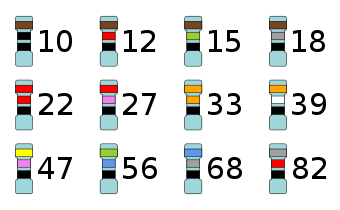
\includegraphics[width=7cm]{fig1.png}
						\caption{E12電阻規格圖}
						\label{fig:fig1}
					\end{center}
				\end{figure}
				而其他誤差的電阻也有其對應的生產規格(如5\%電阻的E12規格),因此並不是所有的電阻色碼都會被製造。	
	\end{enumerate}
\end{enumerate}


\end{document}

